% RLHF Timeline — Key developments across three eras for Chapter 2
% Horizontal timeline with color-coded eras, all labels above in two rows

\documentclass{article}
\usepackage[margin=0.3cm, left=0.6cm, paperwidth=16.5cm, paperheight=5cm]{geometry}
\usepackage{tikz}
\usetikzlibrary{positioning, arrows.meta, calc, backgrounds}
\pagestyle{empty}
\pagecolor{white}

% Era colors
\definecolor{era1}{HTML}{1565C0}   % blue
\definecolor{era1bg}{HTML}{E3F2FD}
\definecolor{era2}{HTML}{E65100}   % orange
\definecolor{era2bg}{HTML}{FFF3E0}
\definecolor{era3}{HTML}{2E7D32}   % green
\definecolor{era3bg}{HTML}{E8F5E9}

\begin{document}

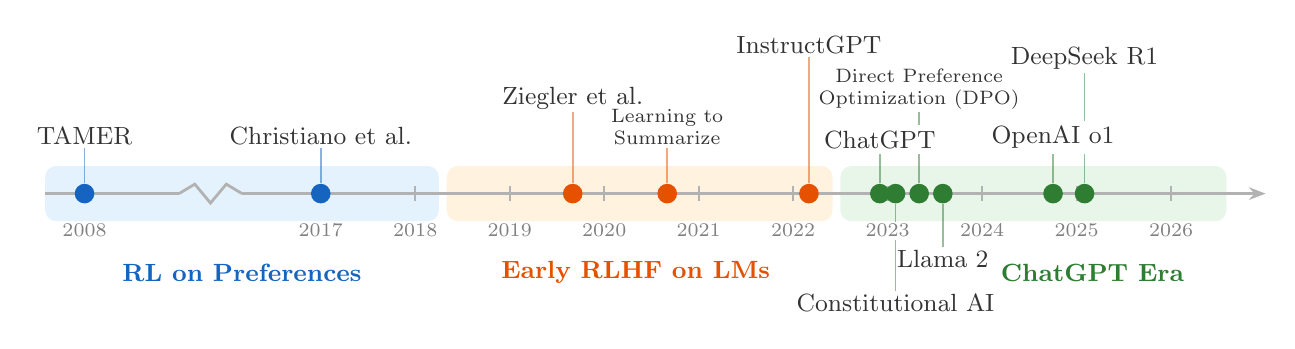
\begin{tikzpicture}[
    milestone/.style={
        circle, fill=#1, inner sep=2.5pt
    },
    row1lbl/.style={
        font=\small, align=center, anchor=south, color=black!80
    },
    row2lbl/.style={
        font=\small, align=center, anchor=south, color=black!80
    },
    eralbl/.style={
        font=\small\bfseries, color=#1
    },
    yearlbl/.style={
        font=\scriptsize, color=black!50, fill=white, inner sep=1pt
    }
]

% Layout: 1.2 units per year from 2017 onward
% 2008=0, break, 2017=3, 2018=4.2, ..., 2025=12.6, 2026=13.8

% Era background bands
\begin{scope}[on background layer]
    \fill[era1bg, rounded corners=4pt] (-0.5, -0.35) rectangle (4.5, 0.35);
    \fill[era2bg, rounded corners=4pt] (4.6, -0.35) rectangle (9.5, 0.35);
    \fill[era3bg, rounded corners=4pt] (9.6, -0.35) rectangle (14.5, 0.35);
\end{scope}

% Timeline axis — left segment, break, right segment with arrow
\draw[line width=1.2pt, color=black!30] (-0.5, 0) -- (1.2, 0);
% Break zigzag
\draw[line width=1.0pt, color=black!30]
    (1.2, 0) -- (1.4, 0.12) -- (1.6, -0.12) -- (1.8, 0.12) -- (2.0, 0);
\draw[-{Stealth[length=6pt]}, line width=1.2pt, color=black!30]
    (2.0, 0) -- (15.0, 0);

% Year ticks (lines only — labels drawn after milestones so they appear on top)
\draw[color=black!30, line width=0.8pt] (0, -0.1) -- (0, 0.1);
\foreach \x in {3, 4.2, 5.4, 6.6, 7.8, 9, 10.2, 11.4, 12.6, 13.8} {
    \draw[color=black!30, line width=0.8pt] (\x, -0.1) -- (\x, 0.1);
}

% -- Milestones (all above, alternating row 1 and row 2) --
% Row 1 (closer): stem 0.35, label at 0.5
% Row 2 (higher): stem 1.1, label at 1.25

% Era 1: blue
% TAMER (2008) — above, row 2
\node[milestone=era1] (tamer) at (0, 0) {};
\draw[era1, line width=0.6pt, opacity=0.5] (tamer.north) -- ++(0, 0.45);
\node[row1lbl] at (0, 0.5) {TAMER};

% Christiano et al. (2017) — row 1, x=3.0
\node[milestone=era1] (christiano) at (3, 0) {};
\draw[era1, line width=0.6pt, opacity=0.5] (christiano.north) -- ++(0, 0.45);
\node[row1lbl] at (3, 0.5) {Christiano et al.};

% Era 2: orange
% Ziegler et al. (Sep 2019) — row 2, x=6.2
\node[milestone=era2] (ziegler) at (6.2, 0) {};
\draw[era2, line width=0.6pt, opacity=0.5] (ziegler.north) -- ++(0, 0.9);
\node[row2lbl] at (6.2, 0.95) {Ziegler et al.};

% Summarize (Sep 2020) — row 1, x=7.4
\node[milestone=era2] (stiennon) at (7.4, 0) {};
\draw[era2, line width=0.6pt, opacity=0.5] (stiennon.north) -- ++(0, 0.45);
\node[row1lbl, font=\scriptsize] at (7.4, 0.5) {Learning to\\Summarize};

% InstructGPT (Mar 2022) — row 3, x=9.2
\node[milestone=era2] (instructgpt) at (9.2, 0) {};
\draw[era2, line width=0.6pt, opacity=0.5] (instructgpt.north) -- ++(0, 1.6);
\node[row2lbl] at (9.2, 1.65) {InstructGPT};

% Era 3: green
% DPO (May 2023) — row 2 above, x=10.2+0.4=10.6 (drawn before ChatGPT so stem is behind)
\node[milestone=era3] (dpo) at (10.6, 0) {};
\draw[era3, line width=0.6pt, opacity=0.5] (dpo.north) -- ++(0, 0.9);
\node[row2lbl, font=\scriptsize] at (10.6, 0.95) {Direct Preference\\Optimization (DPO)};

% ChatGPT (Nov 2022) — row 1 above, x=10.1 (drawn after DPO so label is on top)
\node[milestone=era3] (chatgpt) at (10.1, 0) {};
\draw[era3, line width=0.6pt, opacity=0.5] (chatgpt.north) -- ++(0, 0.45);
\node[row1lbl, fill=white, inner sep=2pt] at (10.1, 0.5) {ChatGPT};

% Constitutional AI (Dec 2022) — below row 2, x=10.3
\node[milestone=era3] (cai) at (10.3, 0) {};
\draw[era3, line width=0.6pt, opacity=0.5] (cai.south) -- ++(0, -1.1);
\node[font=\small, align=center, anchor=north, color=black!80] at (10.3, -1.15) {Constitutional AI};

% Llama 2 (Jul 2023) — below, x=10.2+0.7=10.9
\node[milestone=era3] (llama) at (10.9, 0) {};
\draw[era3, line width=0.6pt, opacity=0.5] (llama.south) -- ++(0, -0.55);
\node[font=\small, align=center, anchor=north, color=black!80] at (10.9, -0.6) {Llama 2};

% DeepSeek R1 (Jan 2025) — row 3, x=12.7 (drawn before o1 so stem is behind)
\node[milestone=era3] (r1) at (12.7, 0) {};
\draw[era3, line width=0.6pt, opacity=0.5] (r1.north) -- ++(0, 1.4);
\node[row2lbl] at (12.7, 1.45) {DeepSeek R1};

% OpenAI o1 (Sep 2024) — row 1, x=12.3 (drawn after DeepSeek so label covers stem)
\node[milestone=era3] (o1) at (12.3, 0) {};
\draw[era3, line width=0.6pt, opacity=0.5] (o1.north) -- ++(0, 0.45);
\node[row1lbl, fill=white, inner sep=2pt] at (12.3, 0.5) {OpenAI o1};

% Year labels (drawn last so they appear in front of stems)
\node[yearlbl, below] at (0, -0.35) {2008};
\foreach \y/\x in {2017/3, 2018/4.2, 2019/5.4, 2020/6.6, 2021/7.8, 2022/9, 2023/10.2, 2024/11.4, 2025/12.6, 2026/13.8} {
    \node[yearlbl, below] at (\x, -0.35) {\y};
}

% Era labels
\node[eralbl=era1] at (2.0, -1.0) {RL on Preferences};
\node[eralbl=era2] at (7.0, -1.0) {Early RLHF on LMs};
\node[eralbl=era3] at (12.8, -1.0) {ChatGPT Era};

\end{tikzpicture}

\end{document}
